 \documentclass[12pt,english]{article}
\usepackage[utf8]{inputenc}
\markright{Pearse et al.\hfill Assessing the Effects Imputation on ED Values\hfill}
\usepackage{geometry}
\geometry{verbose,letterpaper,tmargin=2.54cm,bmargin=2.54cm,lmargin=2.54cm,rmargin=2.54cm}
%\geometry{verbose,letterpaper,tmargin=.1cm,bmargin=.1cm,lmargin=.1cm,rmargin=.1cm}
\usepackage{graphicx}
\DeclareGraphicsExtensions{.pdf,.png,.jpg}
\usepackage{amssymb,amsmath}
\usepackage{epstopdf}
\usepackage{supertabular}
\DeclareGraphicsRule{.tif}{png}{.png}{`convert #1 `dirname #1`/`basename #1 .tif`.png}
\usepackage{url}
\usepackage{subcaption}
\usepackage{caption}
\usepackage[super]{nth}
\usepackage{lineno} \linenumbers
\usepackage[doublespacing]{setspace}
\usepackage[parfill]{parskip}
\setlength{\parindent}{0pt}
\usepackage[citestyle=authoryear,bibstyle=authoryear,sorting=nyt,maxcitenames=2,maxbibnames=10,minbibnames=6,doi=false,url=false,isbn=false,firstinits=true,uniquename=false,uniquelist=false]{biblatex}
\bibliography{edge_sims}
\renewbibmacro*{name:andothers}{% Based on name:andothers from biblatex.def
  \ifboolexpr{
    test {\ifnumequal{\value{listcount}}{\value{liststop}}}
    and
    test \ifmorenames
  }
    {\ifnumgreater{\value{liststop}}{1}
       {\finalandcomma}
       {}%
     \andothersdelim\bibstring[]{andothers}}
    {}}
\renewcommand*{\finalnamedelim}{%
  \ifnumgreater{\value{liststop}}{2}{\finalandcomma}{}%
  \addspace\&\space}
\renewbibmacro{in:}{}
\AtEveryBibitem{%
  \clearfield{day}%
  \clearfield{month}%
  \clearfield{endday}%
  \clearfield{endmonth}%
}
\DeclareFieldFormat[article]{citetitle}{#1}
\DeclareFieldFormat[article]{title}{#1}
\DeclareFieldFormat[article]{pages}{#1}
\DeclareNameAlias{sortname}{last-first}

\usepackage{changes}
\setdeletedmarkup{\textcolor{red}{\sout{#1}}}

\begin{document}
\setlength{\parindent}{0pt}
\section*{Title page}
\textbf{Article type}: Perspectives

\textbf{Article title}: Assessing the Effects Imputation on ED Values

\textbf{Running head}: Assessing the Effects Imputation on ED Values

\textbf{Authors:} K.\ Bodie Weedop$^{1*}$, William D.\ Pearse$^{1*}$\

$^1$ Department of Biology \& Ecology Center, Utah State University,
5305 Old Main Hill, Logan UT, 84322

$^*$To whom correspondence should be addressed:
\url{will.pearse@usu.edu} and \url{bodie.weedop@aggiemail.usu.edu}

\textbf{Word-count}: 5680 (abstract, main text, acknowledgements, and references)

\clearpage
\section*{Abstract}

Some text here.

\textbf{Keywords}: 

\clearpage
\section*{Introduction}
Evidence from the fossil record and present-day studies argue we are
in the midst of, or entering, a sixth mass extinction \autocite{Barnosky2011; Ceballos2015}, such that more species than ever are
declining and/or in danger of extinction across a range of
environments \autocite{Wake2008,Thomas2004}. Habitat destruction
\autocite{Brooks2002}, invasive species
\autocite{Molnar2008}, climate change
\autocite{Pounds2006}, and disease \autocite{Lips2006} are some of
the leading causes of species declines globally. Conservation
biologists seeks to overcome these declines and their detrimental
effects on species populations. Even still, such researchers and
conservationists are confronted with ``Noah's Ark problem''
\autocite{Weitzman1998}, or an unfortunate reality of insufficient,
finite resources to confront the increasing amount species requiring
conservation effort.

Conservation triage has provided an efficient decision making process
for allocating finite resources to obtain the greatest return
\autocite{Bottrill2008}. One of these triage strategies which have been
introduced and used most widely is EDGE \autocite{Isaac2007}. This
method prioritizes species according to two metrics: evolutionary
distinctiveness (ED) and global endangerment (GE). ED measures
relative contributions to phylogenetic diversity made by each species
within a particular clade \autocite{Isaac2007}. Such contributions are
assessed by quantifying the amount of branch length which is unique to
each species within the overall phylogeny. GE values are assessed by
assigning numerical values to each of the World Conservation Union
(IUCN) Red List Categories. As species become increasingly threatened
and are placed into more concerning categories (e.g. from Vulnerable
to Endangered), the GE numerical value increases. Increases in either
ED or GE place a particular species at a higher priority for
conservation effort.

In the event of missing DNA or trait data, species are often difficult
or not able to be placed onto a phylogeny. Even in the face of such
uncertainty and missing data, it is understandable that conservation
biologists want to make prioritizations. However, if we are using a
quantitative method for prioritizing species, we should remain
consistent even when uncertainty arises. To our knowledge, a proper
and efficient method for prioritizing species where there is missing
data is still untested. This issue pertains mainly to the calculation
of ED than GE. The IUCN has collected data on most major clades, and
has a strategy for assigning Red Listing values these species which we
know little information and are considered Data Deficient (DD). IUCN
and other conservation organizations support focus on DD species just
the same as Critically Endangered and Endangered species to ensure
consistency \autocite{Rodrigues2006}. The major area of uncertainty in
phylogenetic prioritisation is phylogenetic data. In the past, missing
species data and poorly resolved trees have been addressed using
imputation \autocite{Collen2011, Isaac2012, Jetz2014}. However, to our knowledge, there has been no systematic
investigation of the efficacy of such imputation, both in terms of the
accuracy with which imputed ED values are estimated, and the effect on
other known species’ scores. Indeed, it is unclear whether any
significant information on ED is gained by imputing species which
cannot be placed on the phylogeny. It is also not well understood how
simply removing missing species, compared to performing imputation,
would effect ED values. It may be that simply excluding missing
species may be less intrusive than imputation. In searching for a
solution for missing species, we may be negatively affecting correct
ED values and disrupting EDGE rankings in the process. As the desire
to use ED and phylogenies for conservation triage grows, the
importance of such tests and a consensus on how to resolve cases of
phylogenetic uncertainty becomes more urgent.

Here, we assess and compare the impact that missing species versus
phylogenetic imputation has upon ED values. In doing so, we hope to
understand the effect that both methods have on ED values and offer a
viable solution for dealing with missing data species. Missing species
were simulated and removed from trees in two ways: randomly and in a
phylogenetically biased manner. Additionally, we tested how ED values
were affected by resolving and imputing polytomies of varying sizes on
a phylogeny. We found that ED values are by removing missing
species. Here is a reference to figure.

\section*{Methods}
We attempted to demonstrate the effects of removing or imputing
species which cannot be placed onto a phylogeny. While assessing the
impact of dropping species and phylogenetic imputations, we were
primarily focused on ED values. In testing the effects on these
values, we remain focused upon ED as a single variable. We exclude GE
because it would only add complexity while not providing any
additional information to our particular investigation.

In each test, we simulated 100 phylogenetic trees and manipulated each
tree’s tips or clade. All simulations, calculations, and analyses were
performed using R (version 3.4.0). Original and manipulated trees were
simulated under a pure-birth Yule model using the sim.bdtree function
‘geiger’ R package \autocite{Harmon2007}. This particular model was
chosen to maintain simplicity. Results from this simple model should
be applicable to other more complex scenarios. Also, to reduce
uncertainty, we used the same model throughout each of the
simulations. In reality, we would be estimating the parameters of the
model which the phylogeny is built upon. The function ed.calc within
the R package ‘caper’ was used to calculate ED values for each tree
\autocite{Orme2013}.

We assessed the impact that removing missing species has upon ED
values using the correlation of all ED values for the tips remaining
within both trees. To evaluate the effect that imputation has upon ED
values, we calculated ED for all tips in both the original and
manipulated trees while excluding the focal clade where imputation has
occurred. These ED values were compared using a
correlation. Additionally, we did the same calculations and comparison
using only the original focal clade and its’ simulated replacement. If
missing species have no effect upon ED values, we expect a high,
positive correlation coefficient between the original tree and its’
manipulated counterpart.

\subsection*{Assessing the impact of missing species on EDGE-listing}
If missing species has a negative effect on ED values, then the
correlation between the ED of the species in the original tree and the
same tree with a fraction of tips removed in some manner should be
significantly different from 1. To investigate the degree of this
effect, we removed tips from simulated trees (Number of taxa = 64,
128, 256, 512, 1024, 2048, 4096) at random and by phylogenetic
clusters. To assess the effect under varying amounts of uncertainty,
fractions of tips dropped ranged from 0 to 0.2 of total tree tips.

Missing species at random was simulated by selecting species at random
without replacing, and removing those species from the tree. This
randomization had no regard for phylogenetic structure. Missing
species related by some character trait was tested by simulating
character trait values for each tip. These simulations were all
performed under a constant rate Brownian-motion model (par = 0.5,
starting root value = 1). Tips were dropped if their character trait
values place them into the upper quantile which had been selected to
be dropped. More specifically, if the fraction to be dropped was 0.1,
species within the 90th quantile of character trait values are
dropped. This is equivalent to Felsenstein’s threshold model
\autocite{Felsenstein2004}.

\subsection*{Assessing the impact of phylogenetic imputations}
We tested the impact of imputing missing species onto a clade of a
particular size (Number of taxa = 2, 3, 4, 8, 16) which originated
from a tree of a particular size (Number of taxa = 64, 128, 256, 512,
1024). To simulate the effect that phylogenetic imputation has upon
these simulated trees, we randomly chose clades within each tree and
treated it as a polytomy to be resolved. The clade selected was
removed from the original tree and a new separate tree of the same
size was simulated under the pure-birth model used before and placed
back where the original clade was removed. By doing this , we
replicated the process of imputation of a clade which has been
resolved. To ensure that this is representative of cases where
imputation is used, 100 repetitions of this simulation were performed
across different parameter settings.

\begin{figure}[!ht]
  \center
  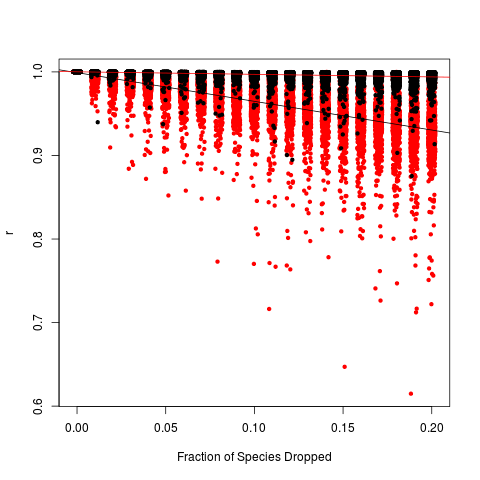
\includegraphics[width=\textwidth]{randomVsCluster.png}
  \caption{\textbf{R-values plotted against the fraction of species 
  dropped at random versus clustered manner.} The color of data points denote 
  whether species were dropped at random (black; n = 100) or in clustered manner 
  (red; n = 100). The regression lines are demonstrating the relationship when 
  species are dropped at random (red) and in a clustered manner (black).}
  \label{randomVsClustered}
\end{figure}

\begin{figure}[!ht]
  \center
  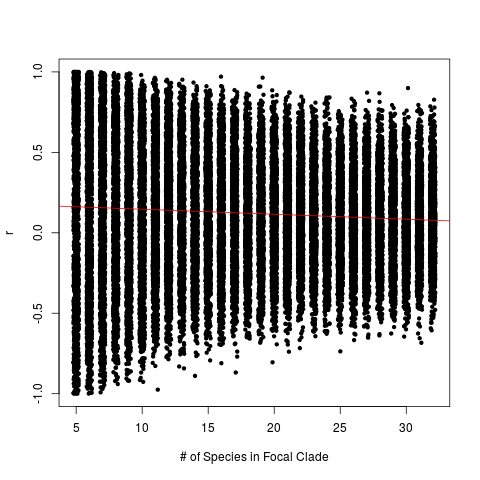
\includegraphics[width=\textwidth]{edModel.png}
  \caption{\textbf{R-values plotted against the number of species at focal clade.} 
  Each data point denotes a correlative comparison between ED values within the focal 
  clades where imputation has occurred. The regression line (red) and trend even closer to zero 
  demonstrates the decrease in informative value of the imputed ED values. This is reinforced 
  by the visual narrowing of r-values around zero.}
  \label{imputationTrend}
\end{figure}

\begin{figure}[!ht]
  \center
  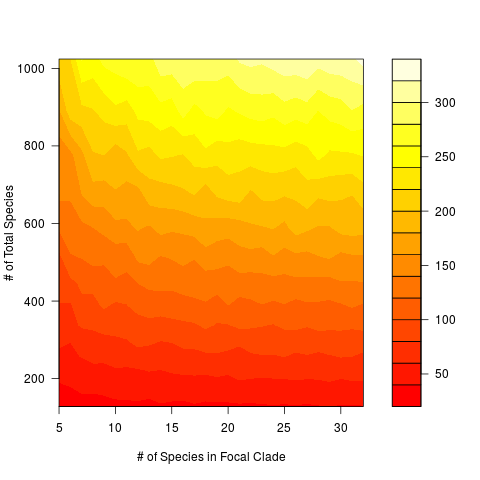
\includegraphics[width=\textwidth]{rankingError.png}
  \caption{\textbf{Mean ranking error of species within the focal clade.} The 
  gradient on the right demonstrates average number of posistions within the 
  full ranking that focal clade species shifted from their true rank.
  While controlling for the size of the full phylogeny and focal clade, species 
  within the focal clade were, on average, ranked far from the true rank. }
  \label{rankingError}
\end{figure}

\section*{Results}
\subsection*{Assessing the impact of missing species on EDGE-listing}

ED values for remaining species were significantly affected by the
fraction of species which were removed (Table 1). However, different
effects are seen when dropping species at random and in clustered
manner (Figure 1). Dropping species at random has a reduced effect
when compared to the effect which dropping species in a clustered
manner has on remaining ED values\ref{randomVsClustered}.

\subsection*{Assessing the impact of phylogenetic imputations}

ED values for the full tree while excluding the focal clade remain at
1 and unaffected. However, ED values for the imputed clades are
significantly affected by the use of imputation. As the size of the
focal clade increases, the informative value of the ED values within the clade 
decreases (Fig. 2)\ref{imputationTrend}. However, even when imputing smaller 
clades, ED values did not regularly reflect the true ED values (Table 2)\ref{imputationModel}.
Additionally, just as imputed ED values did not reflect true ED values, the rankings
of species within the focal clade were altered significantly (Fig. 3)\ref{rankingError}.
ED values outside of the focal clade were not affected by imputation.
While ED values within the focal clades were affected exclusively by imputation, 
a notable error rate in ranking crucial species correctly is present 
(Fig. 1-6S).  


\begin{table}[ht] 
\centering
\begin{tabular}{rrrrr}
  \hline
 & Estimate & Std. Error & t value & Pr($>$$|$t$|$) \\
  \hline
 (Intercept) & 0.1914 & 0.0040 & 48.32 & 0.0000 \\
   clade.size & -0.0036 & 0.0002 & -17.67 & 0.0000 \\
  \hline
  R$^{2}$ & 0.006 \\
  Residual Std. Error & 0.385 (df = 47998) \\
  F Statistic & 312.170$^{***}$ (df = 1; 47998) \\
  \hline
  \hline
\textit{Note:}  & \multicolumn{1}{r}{$^{*}$p$<$0.1; $^{**}$p$<$0.05; $^{***}$p$<$0.01} \\
\end{tabular}
\caption*{\textbf{Table 2: Effect of Clade Size on Imputed ED Values.} The 
intercept describes that the correlation between the true and imputed values 
begins quite low. As the clade size increases, this correlation only tends
toward zero.}
\end{table}

\section*{Discussion}
Some text here.

\section*{Acknowledgments}
\emph{Some text here if needed}.
\clearpage
\printbibliography


\end{document}
%%% Local Variables:
%%% mode: latex
%%% TeX-master: t
%%% End: